\documentclass[11pt]{article}
\usepackage[margin=1in]{geometry}
\usepackage{graphicx}
\usepackage{booktabs}
\usepackage{float}
\usepackage{amsmath,amssymb,url}

\title{Advanced Econometric Methods:sample}
\author{Student ID: Your Student ID\\Your Name}
\date{}
\newcommand{\resultfile}[2]{%
  \IfFileExists{#1}{\input{#1}}{\fbox{\parbox{0.9\linewidth}{#2}}}%
}

\begin{document}
\maketitle

\section*{Question 1}
\subsection*{1.1 Scatter plot}
Figure~\ref{fig:scatter} shows a positive association in simulated data. The line is the least-squares fit.
\begin{figure}[H]
  \centering
  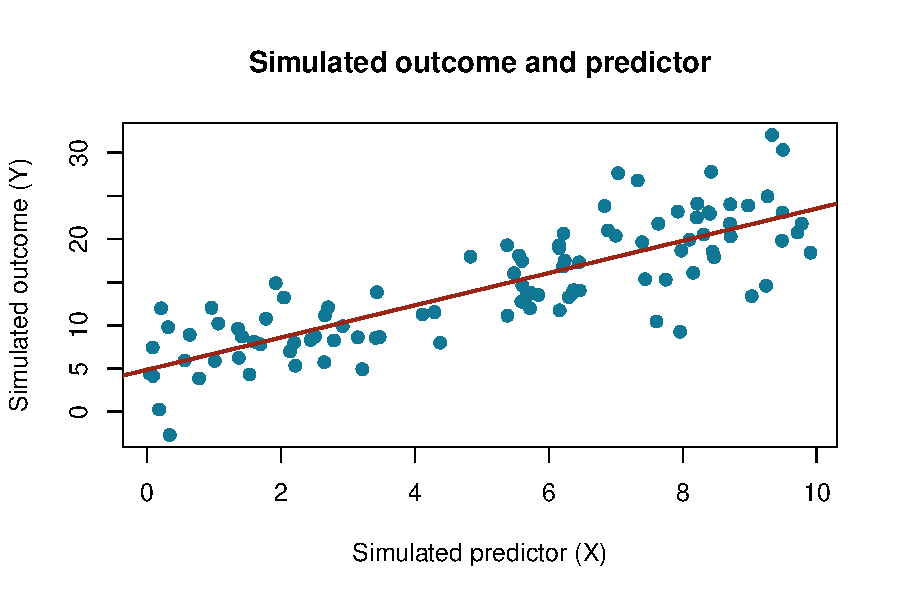
\includegraphics[width=0.72\textwidth]{../output/figures/scatter.pdf}
  \caption{Simulated outcome (Y) and predictor (X), with a least-squares fit.}
  \label{fig:scatter}
\end{figure}

\subsection*{1.2 Event-study}
The event-study simulation assigns treatment to 60 of 120 units. Outcomes include unit and time effects, a rising treatment effect after period 0, and random noise. Period $-1$ is the reference period. Figure~\ref{fig:event-study} plots the estimated two-way fixed-effects coefficients and 95\% confidence intervals; estimates before treatment should be near zero in this simulation.
\[
Y_{it} = \alpha_i + \lambda_t + \sum_{k \neq -1} \tau_k D_i \mathbb{1}\{t = k\} + \varepsilon_{it}.
\]
\begin{figure}[H]
  \centering
  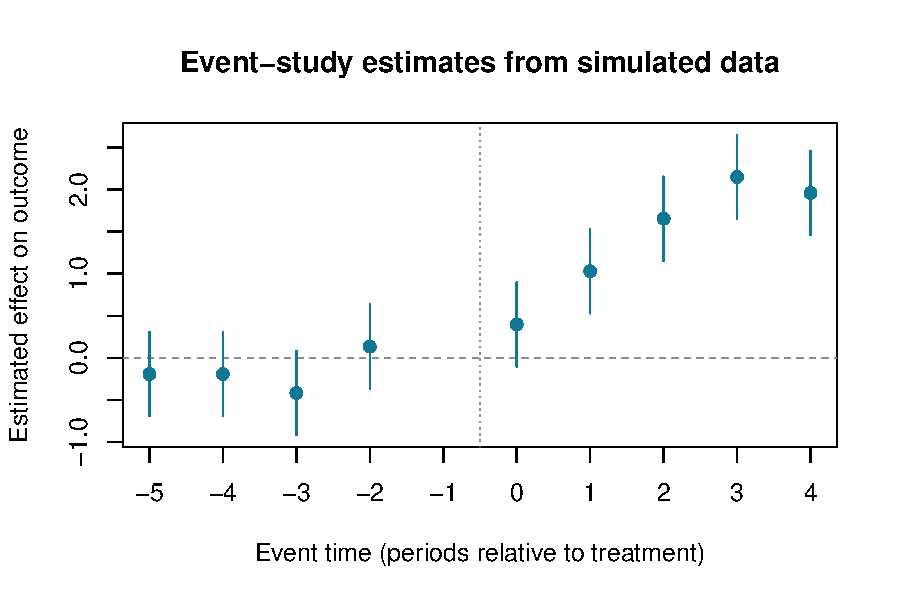
\includegraphics[width=0.72\textwidth]{../output/figures/event_study.pdf}
  \caption{Event-study estimates from the simulated panel; bars show 95\% confidence intervals.}
  \label{fig:event-study}
\end{figure}

\section*{Question 2}
\subsection*{2.1 Penguin figure}
Figure~\ref{fig:penguins} uses the Palmer Penguins data. The panels show bill length by flipper length for each sex, body mass by flipper length, and the flipper-length distributions by species. Records with missing sex or plotted measurements are omitted.
\begin{figure}[H]
  \centering
  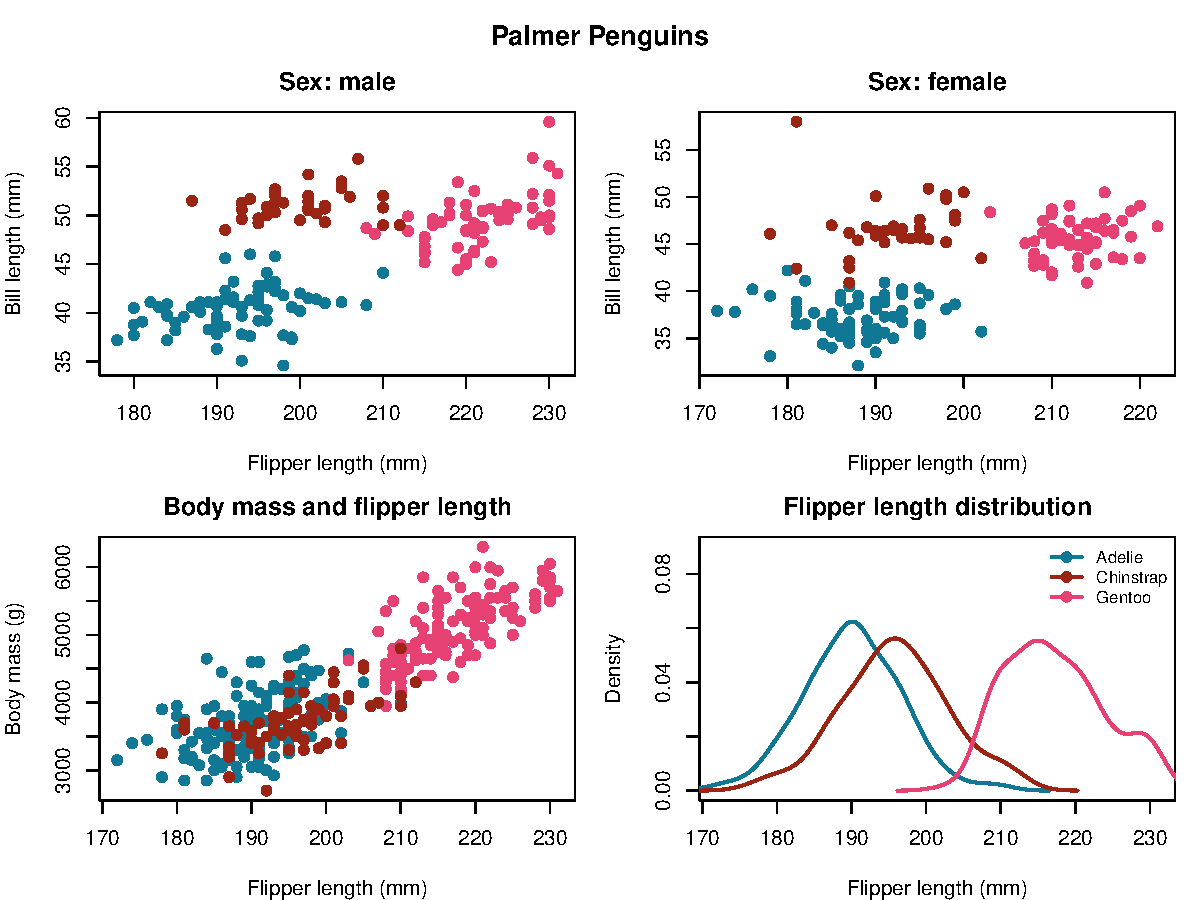
\includegraphics[width=0.95\textwidth]{../output/figures/penguins.pdf}
  \caption{Penguin measurements by sex and species. Source: Horst, Hill, and Gorman (2020).}
  \label{fig:penguins}
\end{figure}

\subsection*{2.2 Table}
Table~\ref{tab:penguins} reports mean bill length, bill depth, flipper length, and body mass by species and sex. Records with missing sex are omitted; each mean uses the available observations for that measurement.
\begin{table}[H]
  \centering
  \caption{Penguin summary statistics by species and sex.}
  \label{tab:penguins}
  \small
  \resultfile{../output/tables/table_penguin_summary.tex}{Run code/analysis.R to create the summary-statistics table.}
\end{table}

\subsection*{2.3 Regression}
We estimate an OLS model of bill length on species, sex, and flipper length. The coefficients are conditional associations, not causal effects. Adelie and female penguins are the reference categories.
\[
\text{Bill length}_i = \beta_0 + \beta_1 \mathbb{1}\{\text{Chinstrap}_i\} + \beta_2 \mathbb{1}\{\text{Gentoo}_i\} + \beta_3 \mathbb{1}\{\text{Male}_i\} + \beta_4 \text{Flipper length}_i + \varepsilon_i.
\]
The regression table below reports the OLS estimates.
\begin{table}[H]
  \centering
  \caption{OLS estimates for penguin bill length.}
  \label{tab:penguin-regression}
  \small
  \resultfile{../output/tables/table_penguin_regression.tex}{Run code/analysis.R to create the regression table.}
\end{table}
\noindent The table reports conventional OLS standard errors in parentheses, the outcome mean, sample size, and R-squared. The sample contains complete cases for the variables in the regression.

\noindent $^{*}p<0.10$, $^{**}p<0.05$, and $^{***}p<0.01$.

\noindent Horst, A. M., Hill, A. P., \& Gorman, K. B. (2020). \textit{palmerpenguins: Palmer Archipelago (Antarctica) penguin data} (R package version 0.1.0) [Data set]. Zenodo. \url{https://doi.org/10.5281/zenodo.3960218}
\end{document}
